\chapter{TLS}

\section{Original SSL (Secure Socket Layer)}
Secure transport channel originally proposed by Netscape Communications in 1995, it have has the following characteristics:
\begin{itemize} 
    \item \textbf{Peer authentication} (server, server+client) $\rightarrow$ asymmetric challenge-response (implicit, explicit)
    \item \textbf{Message confidentiality} $\rightarrow$ symmetric encryption
    \item \textbf{Message authentication and integrity} $\rightarrow$ MAC computation
    \item \textbf{Protection against replay, filtering, and reordering attacks} $\rightarrow$ implicit record number (used in MAC computation!) plus 
    layering on TCP -> \textbf{For exam} tell that the record number is also included in the computation of the MAC
\end{itemize}

\section{TLS achitecture}

\begin{figure}[h!]
    \centering
    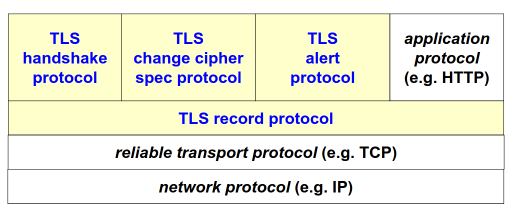
\includegraphics[width=0.5\textwidth]{img/tls_arch.png}
    \caption{Arch TLS}
    \label{fig:tls_arch}
\end{figure}

\begin{itemize}
    \item one \textbf{network protocol}, typically nowadays IP, but that is not compulsory (Anything at layer 3 can work)
    \item  a reliable \textbf{transport protocol}, For example, TCP.
    \item Then the \textbf{TLS record protocol}: a generic protocol just for transporting things between the two peers. \\
            First it transport the \textbf{TLS handshake protocol}, then the \textbf{ChangeCypherSpec} (When you need to change from one algorithm to another, and notably from no protection to protection),
            when something bad happens  one last message, which is part of the \textbf{alert protocol} (and then close the connection). If everything is going well, the record protocol is used to transport some \textbf{application protocol}.

    
\end{itemize}

\section{TLS sessions and connections}

In a \textbf{TLS session}, created by the handshake protocol, is a a logical association betweeen the client and server that agree on a set of cryptographic parameters (is shared between different connections 1:N) \\

A  \textbf{TLS connection} is the transient TLS channel between the client and server, and is associated with a session. \\

\section{TLS handshake protocol}
Used to agree in a set of algorithms for confindentality, integrity. During the handshake are exchange random numbers between the client and the server to be used for the subsequent generation of the keys, use to establish a symmetric key by means of public key operations (RSA, DH, ...). \\ 
In the end are also negotiate the session-id and exchanged the necessary certificates.

\newpage
\section{Data protection}

\begin{figure}[!ht]
    \centering
    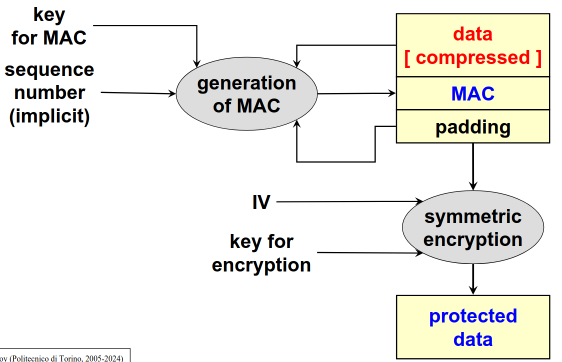
\includegraphics[width=0.5\textwidth]{img/data_protection.png}
    \caption{Authenticate then encrypt}
    \label{fig:data_prot}
\end{figure}
\begin{itemize}
    \item In authenticate-then-encrypt data that are coming from the application layer. Until TLS 1.2 it was possible to compress those data before transmitting and the negotiation also of compression algorithm was part of the handshake. (Can lead to attack so in new version of TLS is not possible to compress data)
    \item The keys are not unique, but are directional (one for encrypt server to client, and one for encrypt client to server). This is done because, is used the number of the packet in the sequence for accept it or not, and if the key is the same one part can copy a packet with id X and sent it back when his sequence arrive at the same number. 
\end{itemize}


\section{Relationship among key and sessions}

\begin{figure}[h!]
    \centering
    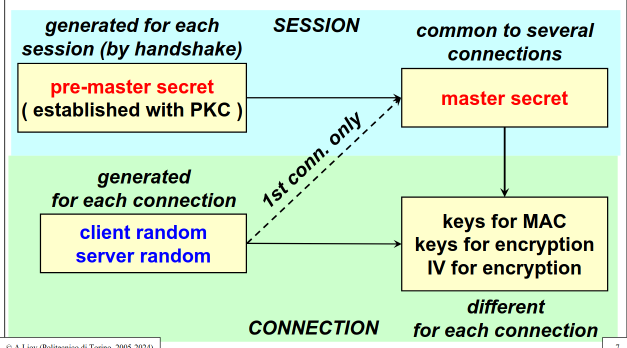
\includegraphics[width=0.5\textwidth]{img/key_sess.png}
    \label{fig:key_session}
\end{figure}

The only value common at each connection is the master key used for generate keys for enc and IV.
(all other value keys, iv are unique for each connection). \\
Every time you open a new channel, there are new client and server random that are used together with the master secret to create the specific keys for that connection.

\subsection{Problem}
Since the key material is generated starting from a symmetric crypto, we have a problem. If the private key used for performing encryption and decryption of the pre-master secret is discovered, then if someone has made a copy of all the past traffic, will now be \textbf{able to decrypt all the traffic} (present, past and future). \\
We would like very much to have a specific property which is named perfect forward secrecy.

\section{Perfect forward secrecy (PFS)}
Perfect Forward Secrecy ensures that even if the session key used for key exchange is compromised, only current and eventually future communications are at risk, while past communications remain secure.

\subsection{Ephemeral mechanisms}
An ephemeral key exchange mechanism is used to generate a new session key on the fly, that need to be signed with the long term private key ( but cannot have an associated X.509 certificate because the CA process is slow and often not on-line). \\ Usually used for Diffie-Hellman (DH) but is slow in RSA. \\

SO, we have the server’s private key used only for signing and we obtain
a perfect forward secrecy. \\
\begin{itemize}[itemsep=0pt]
    \item  If the (temporary or short-lived) private key is compromised
          then the attacker can decrypt only the related traffic
    \item Compromise of the long-term private key is an issue for
          authentication but not for confidentiality
\end{itemize}

!! Valutare immagini slide 10 e 11 !!

...

\begin{figure}[h!]
    \centering
    \subfigure[Image 1]{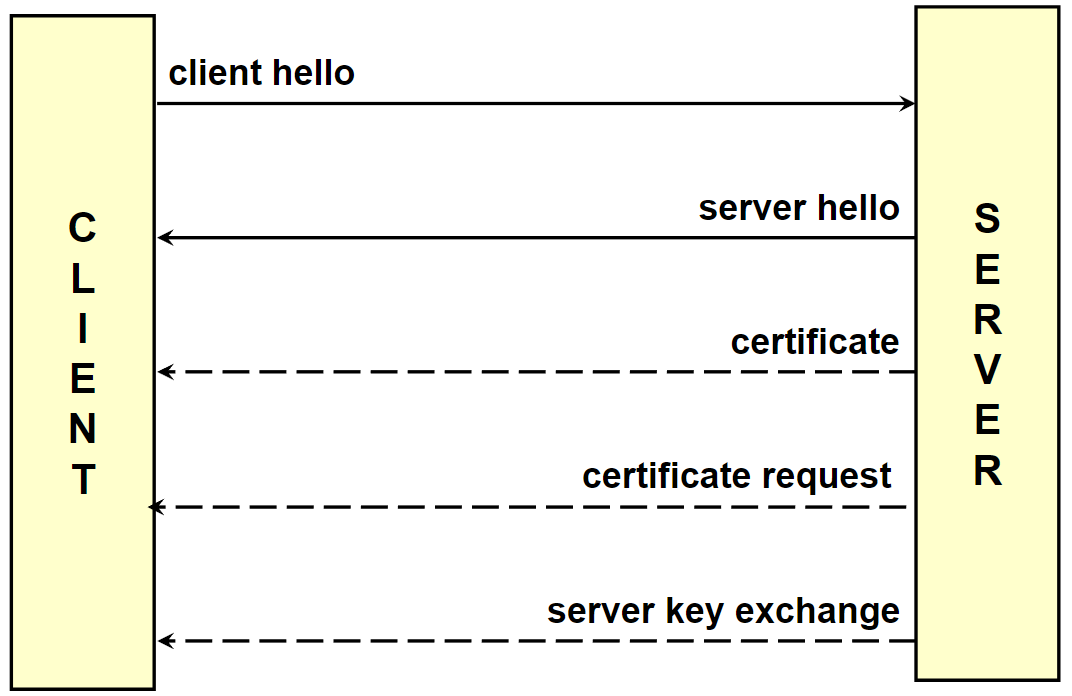
\includegraphics[width=0.45\textwidth]{img/ephemeral1.png}}
    \hfill
    \subfigure[Image 2]{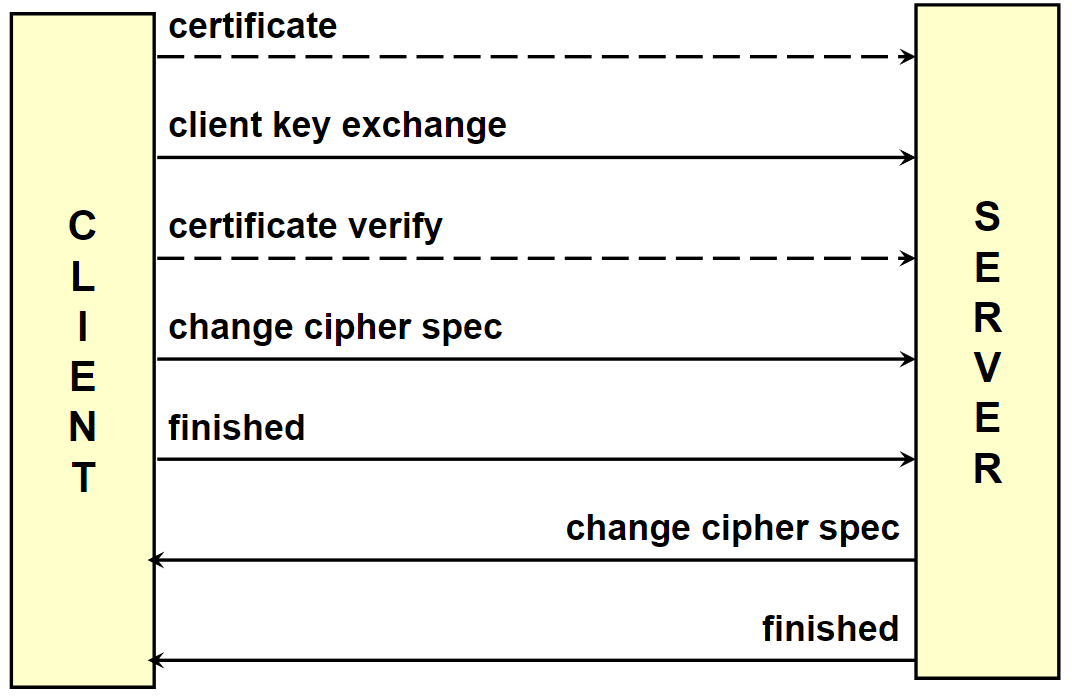
\includegraphics[width=0.45\textwidth]{img/ephemeral2.png}}
    \caption{Steps of ephemeral key exchange}
    \label{fig:two_images}
\end{figure}

\subsubsection{Client Hello}

In the "Client Hello" message, the client begins by specifying its preferred SSL/TLS version, indicating the highest version it supports (e.g., 2 for SSL-2, 3.0 for SSL-3, 3.1 for TLS-1.0). It also includes 28 pseudo-random bytes known as the "Client Random," and a session identifier (session-id). (If the session-id is 0 $\rightarrow$ requested a new session. Non-zero value $\rightarrow$ resume a previous session). The message also contains a list of supported cipher suites, which define the algorithms for encryption, key exchange, and integrity, and a list of supported compression methods.

\subsubsection{Server Hello}

In the "Server Hello" message, the server responds by selecting the SSL/TLS version to use. It then sends 28 pseudo-random bytes known as the "Server Random" and provides a session identifier. If the session-id in the client hello was 0, the server generates a new session-id or rejects the session-id proposed by the client. If the server accepts the session resumption request, it echoes the session-id provided by the client. The server also selects the strongest cipher suite that is common with the client, and it specifies the compression method to be used.

\subsubsection{Cipher suite}

\begin{itemize}[itemsep=0pt]
    \item key exchange algorithm
    \item symmetric encryption algorithm
    \item hash algorithm (for MAC)
    \item examples:
          \begin{itemize}[itemsep=0pt]
              \item SSL\_NULL\_WITH\_NULL\_NULL
              \item SSL\_RSA\_WITH\_NULL\_SHA
              \item SSL\_RSA\_EXPORT\_WITH\_RC2\_CBC\_40\_MD5
              \item SSL\_RSA\_WITH\_3DES\_EDE\_CBC\_SHA
          \end{itemize}
          \href{https://www.iana.org/assignments/tls-parameters/tls-parameters.xhtml#tls-parameters-4}{complete list maintained by IANA}
\end{itemize}


\subsubsection{Certificate (server)}

In the \textbf{"Certificate"} message from the server, a certificate is provided for \textbf{server authentication}. The certificate's \textbf{subject} or \textbf{subjectAltName} must match the server's identity, such as its \textbf{DNS name} or \textbf{IP address}. The server must send the \textbf{entire certificate chain} up to a trusted root, though the root CA itself should not be included. \\ The certificate can be used for \textbf{signing}, or both \textbf{signing and encryption}, as specified in the \textbf{keyUsage} field. \\ If the certificate is only for signing, a separate \textbf{server key exchange} phase is required to exchange the ephemeral key.

\subsubsection{Certificate Request}

\begin{itemize}[itemsep=0pt]
    \item used for client authentication
    \item specifies also the list of CAs considered trusted by the
          server
          \begin{itemize}[itemsep=0pt]
              \item the browsers show to the users (for a connection) only the
                    certificates issued by trusted CAs
          \end{itemize}
\end{itemize}

\subsubsection{Server key exchange}
The \textbf{Server Key Exchange} message is used to carry the server's public key for key exchange. It is required in the following cases:

\begin{itemize}[itemsep=0pt]
    \item The RSA server certificate is usable only for \textbf{signature}.
    \item \textbf{Anonymous} or \textbf{ephemeral Diffie-Hellman (DH)}
          is used to establish the pre-master secret.
    \item There are \textbf{export restrictions} requiring the use of ephemeral RSA/DH keys.
    \item \textbf{Fortezza ephemeral} keys are used.
\end{itemize}

This message is \textbf{explicitly signed by the server}, and it is important to note that it is the \textbf{only message} in the handshake process that is explicitly signed by the server.

\subsubsection{Certificate (client)}
This message carries the certificate for client authentication. The certificate must have been issued from one of the CAs in the trusted CA list specified in the Certificate Request message.


\subsubsection{Client key exchange}

The client generates material for symmetric keys derivation and sends it to the server in varius ways:
\begin{itemize}
    \item pre-master secret encrypted with the server RSA public key
          (ephemeral or from its X.509 certificate)
    \item client's public part of DH
    \item client's Fortezza parameter
\end{itemize}

\subsubsection{Certificate verify}
The \textbf{Certificate Verify} message involves an explicit test signature performed by the client. In this phase, a hash is computed over all the previous handshake messages and is then encrypted using the client's private key. This step is required only when \textbf{client authentication} is used, allowing the server to identify and reject fake clients.

\subsubsection{Change cipher spec}
The \textbf{Change Cipher Spec} message signals the switch to the newly negotiated algorithms for message protection. It transitions from unprotected messages to encrypting subsequent messages using the agreed-upon algorithms and keys. \\ While it is theoretically considered a separate protocol from the handshake, some analyses suggest that it could potentially be \textbf{eliminated} from the process.

\subsubsection{Finished}

The \textbf{Finished} message is the first message protected with the negotiated algorithms. It plays a crucial role in authenticating the entire handshake process. \\ The message contains a \textbf{MAC} computed over all the previous handshake messages (excluding the \textbf{Change Cipher Spec}), using the \textbf{master secret} as the key. This ensures the integrity of the handshake and prevents rollback \textbf{man-in-the-middle attacks} such as version or cipher suite downgrade. The \textbf{Finished} message is different for the client and server, with each calculating their own MAC.


\section{TLS Comparison}

- TLS, no ephemeral key, no client auth \\
- TLS, no ephemeral key,  client auth \\
- TLS, ephemeral key, no client auth \\
- TLS, data exchange and link teardown \\
- TLS, resumed session

!! immagini da slide 23 a 27, valutare se inserirle !!

\section{TLS setup time}

The \textbf{TLS setup time} involves both the TCP and TLS handshakes.
First, a \textbf{TCP handshake} is performed, followed by the \textbf{TLS handshake}.
Multiple TLS messages can fit within a single TCP segment. Typically, this setup requires
\textbf{1-RTT} for TCP and \textbf{2-RTT} for TLS:

\begin{itemize}[itemsep=0pt]
    \item (C $>$ S) \textbf{SYN}
    \item (S $>$ C) \textbf{SYN-ACK}
    \item (C $>$ S) \textbf{ACK} + \textbf{ClientHello}
    \item (S $>$ C) \textbf{ServerHello} + \textbf{Certificate}
    \item (C $>$ S) \textbf{ClientKeyExchange} + \textbf{ChangeCipherSpec} + \textbf{Finished}
    \item (S $>$ C) \textbf{ChangeCipherSpec} + \textbf{Finished}
\end{itemize}

After around \textbf{180 ms} (assuming a 30 ms one-way delay),
the client and server are ready to exchange protected data.

\section{TLS versions}

\subsection{TLS 1.0 (SSL 3.1)}
\textbf{Transport Layer Security} (TLS) is a standard defined by the IETF, with \textbf{TLS 1.0} specified in \textit{RFC 2246} (January 1999). TLS 1.0 is also known as \textbf{SSL 3.1}, sharing a 99\% similarity with SSL 3. \\
This version places a strong emphasis on using standard (i.e., non-proprietary) digest and asymmetric cryptographic algorithms, which are mandatory.
The required algorithms include \textbf{Diffie-Hellman (DH)}, \textbf{Digital Signature Algorithm (DSA)}, and \textbf{3DES} for encryption, as well as \textbf{HMAC-SHA1} for message authentication.\\ That lead to the ciphersuite \textit{TLS\_DHE\_DSS\_WITH\_3DES\_EDE\_CBC\_SHA}.

\subsection{TLS 1.1}
\textbf{TLS 1.1} is defined in \textit{RFC 4346} (April 2006) and introduces several enhancements to improve security. To protect against \textbf{Cipher Block Chaining (CBC)} attacks, the implicit initialization vector (IV) is replaced with an explicit IV. \\ Additionally, padding errors now trigger the \textbf{bad\_record\_mac} alert message instead of the previous \textbf{decryption\_failed} alert (This is for give less information to an attacker that is trying a padding oracle attack). \\ The update also establishes IANA registries for various protocol parameters. Notably, premature session closes no longer result in sessions being non-resumable, allowing for improved session management.\\ Furthermore, TLS 1.1 includes additional notes addressing various new attack vectors.

\subsection{TLS 1.2}
\textbf{TLS 1.2} is specified in \textit{RFC 5246} (August 2008) and introduces significant improvements in cryptographic functions and security features. One of the key enhancements is that the ciphersuite now specifies the \textbf{pseudo-random function (PRF)} used in the protocol. TLS 1.2 extensively employs \textbf{SHA-256} for various operations, including the \textbf{Finished} message and HMAC. \\ The protocol also adds support for \textbf{authenticated encryption}, utilizing \textbf{AES} in GCM or CCM mode. Additionally, TLS 1.2 incorporates protocol extensions from \textit{RFC 4366} and the AES ciphersuite from \textit{RFC 3268}. \\
The default ciphersuite is \textit{TLS\_RSA\_WITH\_AES\_128\_CBC\_SHA}, while older ciphersuites such as \textbf{IDEA} and \textbf{DES} have been deprecated.


\section{TLS evolution}
\subsection{Ciphersuites and Encryption} The evolution of TLS has introduced various ciphersuites and encryption algorithms. Notable encryption algorithms include:
\begin{itemize}[itemsep=0pt]  
    \item \textbf{AES} specified in \textit{RFC 3268} 
    \item \textbf{ECC} (Elliptic Curve Cryptography) introduced in \textit{RFC 4492} 
    \item \textbf{Camellia} defined in \textit{RFC 4132} 
    \item \textbf{SEED} as outlined in \textit{RFC 4162} \item \textbf{ARIA} specified in \textit{RFC 6209} \end{itemize} In terms of authentication, the following methods have been integrated: \begin{itemize}[itemsep=0pt]  
        \item \textbf{Kerberos} as described in \textit{RFC 2712} 
        \item \textbf{Pre-shared Key} (secret, DH, RSA) introduced in \textit{RFC 4279} 
        \item \textbf{SRP} (Secure Remote Password) detailed in \textit{RFC 5054} 
        \item \textbf{OpenPGP} specified in \textit{RFC 6091} 
    \end{itemize}

\subsection{Compression and Other Features} 
The TLS evolution also includes advancements in compression methods: 
\begin{itemize}[itemsep=0pt] 
    \item Compression methods and \textbf{Deflate} defined in \textit{RFC 3749} 
    \item Protocol compression using \textbf{LZS} as per \textit{RFC 3943} 
\end{itemize} Additionally, several other protocols and extensions have been established: 
\begin{itemize}[itemsep=0pt]
        \item \textbf{Extensions} (specific and generic) as specified in \textit{RFC 4366} 
        \item \textbf{User mapping extensions} detailed in \textit{RFC 4681} 
        \item \textbf{Renegotiation indication extensions} outlined in \textit{RFC 5746} 
        \item \textbf{Authorization extensions} described in \textit{RFC 5878} 
        \item Prohibition of \textbf{SSL 2.0} as per \textit{RFC 6176} 
        \item \textbf{Session resumption} without server state as outlined in \textit{RFC 4507} 
        \item \textbf{Handshake with supplemental data} specified in \textit{RFC 4680} 
\end{itemize}


!! vedere attacchi da slide 34 a 41 !!
\section{Attacks}

\subsection{Heartbleed}
The \textbf{Heartbleed} vulnerability is tied to the \textbf{RFC 6520}, which defines the TLS/DTLS heartbeat extension. This extension was designed to keep a connection alive without the need for constant renegotiation of the SSL session, particularly useful for \textbf{DTLS} (Datagram TLS) and in \textbf{Path Maximum Transmission Unit (PMTU)} discovery.

However, the vulnerability, assigned \textbf{CVE-2014-0160}, stems from a bug in OpenSSL. Due to a \textbf{buffer over-read} issue, the TLS server may send back more data (up to 64kB) than originally requested in the heartbeat message. This can expose sensitive data from the server's RAM, such as user credentials (username and password) or even the server's private key—if the key is not stored in a secure hardware module like an \textbf{HSM} (Hardware Security Module).

\subsection{Bleichenbacher attack (and ROBOT)}
In \textbf{1998}, \textbf{Daniel Bleichenbacher} introduced the so-called "million-message attack," a cryptographic vulnerability targeting the way \textbf{RSA encryption} was implemented. By sending approximately a million specially crafted messages to a server, an attacker could deduce the server's \textbf{private key} through subtle differences in the returned \textbf{error codes}.

Over the years, this attack has been refined to require far fewer messages—in some cases, just thousands—making it feasible to execute from a laptop. In \textbf{2017}, the \textbf{ROBOT (Return Of Bleichenbacher’s Oracle Threat)} attack, a variant of the original, emerged and affected major websites, including \textbf{facebook.com}.

\subsection{Other minor attacks}
\begin{itemize}
    \item \textbf{CRIME} (2012)
    \begin{itemize}
        \item Attacker can:
        \begin{enumerate}
            \item Inject chosen plaintext in user requests
            \item Measure the size of the encrypted traffic
        \end{enumerate}
        \item Exploits information leaked from compression to recover specific plaintext parts.
    \end{itemize}

    \item \textbf{BREACH} (2013)
    \begin{itemize}
        \item Deduces a secret within HTTP responses from a server that:
        \begin{enumerate}
            \item Uses HTTP compression
            \item Inserts user input into HTTP responses
            \item Contains a secret (e.g., CSRF token) in the HTTP responses
        \end{enumerate}
    \end{itemize}

    \item \textbf{BEAST} (Browser Exploit Against SSL/TLS) 2011
    \begin{itemize}
        \item SSL channel using CBC with IV concatenation
        \item A MITM attacker may decrypt HTTP headers with a blockwise-adaptive chosen-plaintext attack
        \item Attacker may decrypt HTTPS requests and steal session cookies or other information.
    \end{itemize}

    \item \textbf{POODLE} (Padding Oracle On Downgraded Legacy Encryption)
    \begin{itemize}
        \item A MITM attack that exploits SSL-3 fallback to decrypt data.
        \item Dec 2014 variant: Exploits CBC errors in TLS 1.0–1.2, so it works even if SSL-3 is disabled.
    \end{itemize}

    \item \textbf{FREAK} (Factoring RSA Export Keys) 2015
    \begin{itemize}
        \item Downgrade to export-level RSA keys (512-bit) and factorize to decrypt the channel.
        \item Alternatively, downgrade to export-level symmetric keys (40-bit) and brute-force the key.
    \end{itemize}
\end{itemize}

\subsection{Freak phases}

\begin{figure}[htbp]
    \centering
    \subfigure[Image 1]{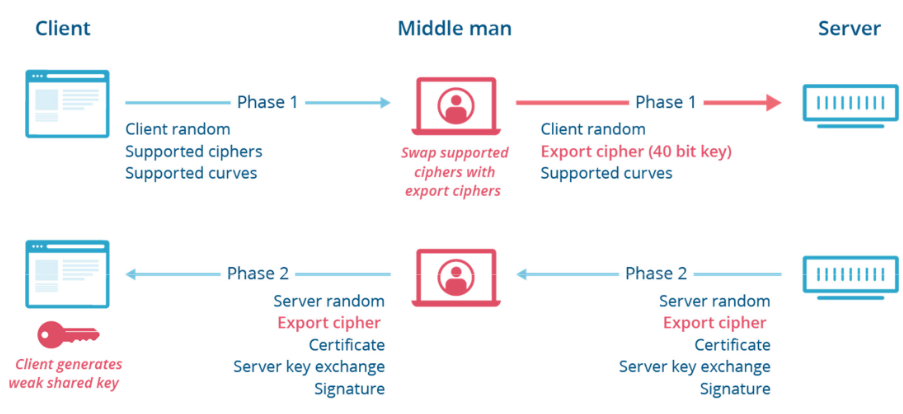
\includegraphics[width=0.45\textwidth]{img/freak1.png}}
    \hfill
    \subfigure[Image 2]{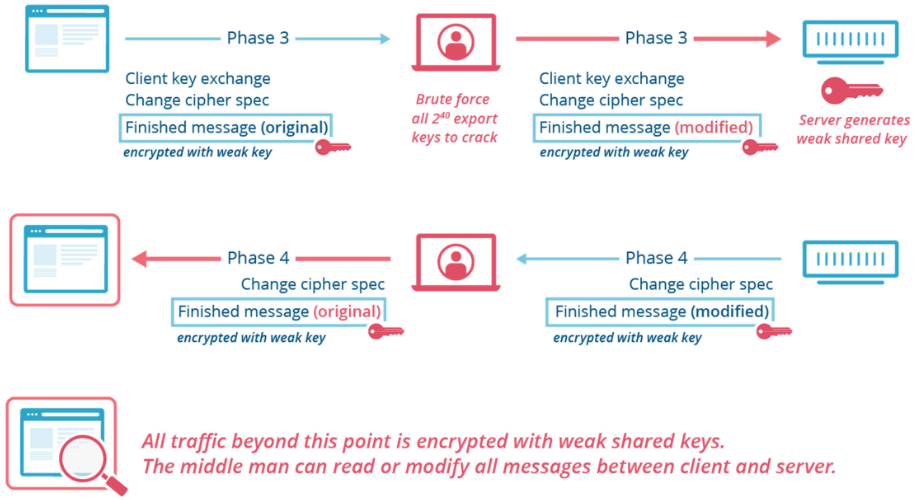
\includegraphics[width=0.45\textwidth]{img/freak2.png}}
    \caption{Freak Attack step by step}
    \label{fig:freak}
\end{figure}


\section{ALPN extension (Application-Layer Protocol Negotiation)}

is an extension that can be added to tls message and give the possibility to negotitate the application layer protocol to use to speed up the connection creation, avoiding additional round-trips for application negotiation: \\
\begin{itemize}
    \item (ClientHello) ALPN=true + list of supported app. protocols
    \item (ServerHello) ALPN=true + selected app. protocol
\end{itemize}
Important for the negotiaton of the HTTP/2 (for FX and chrome is onlt over TLS) and QUIC protocol, but also useful also for those servers that use different certificates for the different application protocols. \\

possible value: http/1.0, http/1.1, h2 (HTTP/2 over TLS), h2c (HTTP/2 over TCP)

\section{TLS False Start}

Another extension, whit it he client can send application data together with the ChangeCipherSpec and Finished messages, in a single segment, without waiting for the corresponding server messages. \\
This lead to recude the latency to 1-RTT, but even if it can work without changes, chome and FX require ALPN + forware secrecy. Safari only require forwared secrecy. \\ 
For enable it, the server must advertise the supported protocols and be configured to prefer cipher suites with forward secrecy. 

\section{The TLS Downgrade Problem}

During a TLS handshake, the client sends (via \textbf{ClientHello}) the highest TLS version it supports. The server then replies (in \textbf{ServerHello}) with the version it will use, which is the highest version supported by both the client and server. In a typical scenario of version negotiation, both parties may agree on \textbf{TLS 1.2}:

\begin{itemize}
    \item Client to Server: 3,3 (indicating TLS 1.2)
    \item Server to Client: 3,3 (agreement on TLS 1.2)
\end{itemize}

If the server does not support \textbf{TLS 1.2}, a fallback to \textbf{TLS 1.1} occurs:

\begin{itemize}
    \item Client to Server: 3,3 (requests TLS 1.2)
    \item Server to Client: 3,2 (fallback to TLS 1.1)
\end{itemize}


In some cases, servers do not respond correctly, potentially closing the connection instead of negotiating the correct version. This forces the client to retry the handshake with a lower protocol version. This behavior can be exploited in a \textbf{downgrade attack}, where an attacker sends a fake server response to force multiple downgrades. Eventually, this may result in the connection being established using a vulnerable version (e.g., \textbf{SSL 3.0}), which could then be exploited with an attack like \textbf{Poodle}. Although downgrades do not always signify an attack, they present security risks when exploited maliciously. \\

\section{TLS Fallback Signalling Cipher Suite Value (SCSV)}

Used for prevents protocl downgrade attacks. It introduce a new dummy chipersuire \textbf{TLS\_FALLBACK\_SCSV} that is used by the client to signal to the server that the connection is a downgraded connection. \\
The server can respond with a new fatal Alert \textbf{in\_appropriate\_fallback} and close the connection if it recive TLS\_FALLBACK\_SCSV and a version lower than the highest one supported. At this point the client can retry the connection with the highest version supported. \\

\subsection{Notes}
It's not support by a lot of server, but most servers have fixed their bad behaviour when the client requests a version higher than the supported one so browsers can now disable insecure downgrade

\section{TLS session tickets}

Another improvment in TLS, that allow the server to send the session datat to the client (to reduce the cache on the server). \\
The session data in the client is:
\begin{itemize}
    \item encrypted with a server secret key
    \item returned to the server when resuming the session
    \item it just move the session ache to the client
\end{itemize}
There are some issues:
\begin{itemize}
    \item needs support at the browser (it's an extension)
    \item in a load balancing environment, it requires key sharing among the various end-points (and periodic key update!)
\end{itemize}


\section{TLS and virtual servers}

A virtual server is a server with a single IP address and multiple domain names associated to it. \\
It'e easy to manage in HTTP/1.1 because in the headerthere is the host field that specify the domain name. \\

\subsection{The problem}
In https it's difficult because TLS is activated before HTTP, so there is no way to know that certificare use.

\subsection{The solution}

\begin{itemize}
    \item \textbf{Collective (wildcard) certificate}: A single certificate covers multiple subdomains, e.g., \texttt{CN=*.myweb.it}, with the private key shared among all servers. However, different browsers may handle wildcard certificates differently.
    
    \item \textbf{Certificate with a list of servers in subjectAltName}: This method includes a list of servers within the \texttt{subjectAltName} field of the certificate, with the private key shared across servers. A drawback is that the certificate needs to be reissued whenever a server is added or removed.
    
    \item \textbf{SNI (Server Name Indication)}: The \texttt{Server Name Indication} (SNI) extension, included in the \textbf{ClientHello} message (as per \textit{RFC 4366}), allows specifying which server the client is trying to reach. However, SNI has limited support among certain browsers and servers.
\end{itemize}

\section{TLS 1.3}

The goals of TLS 1.3 are to:
\begin{itemize}[itemsep=0pt]
    \item reducing handshake latency
    \item encrypting more of the handshake (for security and privacy)
    \item improving resiliency to cross-protocol attacks
    \item removing legacy features
\end{itemize}

\subsection{ key exchange}

TLS 1.3 introduced significant changes to the key exchange process to improve security:

\begin{itemize}
    \item \textbf{Removal of static RSA and DH key exchange}: These methods were eliminated because they do not provide forward secrecy. They also introduced vulnerabilities such as the \textbf{Heartbleed} attack and were difficult to implement correctly. Additionally, they were susceptible to the \textbf{Bleichenbacher attack} (and its variant, \textbf{ROBOT}).
    
    \item \textbf{Use of DHE (Diffie-Hellman Ephemeral)}: TLS 1.3 exclusively uses \textbf{DHE} for key exchange but restricts the use of arbitrary parameters to prevent attacks. For example:
        \begin{itemize}[itemsep=0pt]
            \item \textbf{LogJam (2015)} tricked servers into using weak DH parameters (512-bit).
            \item \textbf{Sanso (2016)} found that OpenSSL generated DH values without the required mathematical properties.
        \end{itemize}
    
    \item \textbf{Predefined groups}: To mitigate these risks, TLS 1.3 uses only \textbf{DHE} with a few predefined, secure groups, ensuring better protection against cryptographic attacks.
\end{itemize}


\subsection{message protection}

TLS 1.3 addressed several vulnerabilities from earlier versions by improving message protection and cryptographic methods:

\subsubsection{Previous Pitfalls}
\begin{itemize}
    \item \textbf{CBC mode and authenticate-then-encrypt}: These techniques were vulnerable to attacks like \textbf{Lucky13}, \textbf{Lucky Microseconds}, and \textbf{POODLE}.
    \item \textbf{RC4 usage}: In 2013, researchers demonstrated that \textbf{RC4} could expose plaintext due to measurable biases in its output.
    \item \textbf{Compression}: The use of compression in TLS was a factor in the \textbf{CRIME} attack, which exploited compressed data to leak information.
\end{itemize}

\subsubsection{TLS 1.3 Improvements}
\begin{itemize}
    \item TLS 1.3 no longer uses \textbf{CBC} or authenticate-then-encrypt schemes. Instead, it only permits \textbf{AEAD} (Authenticated Encryption with Associated Data) modes, which offer strong integrity and confidentiality.
    \item Deprecated older cryptographic methods such as \textbf{RC4}, \textbf{3DES}, \textbf{Camellia}, \textbf{MD5}, and \textbf{SHA-1}.
    \item Compression is no longer used in TLS 1.3, preventing compression-related attacks.
    \item Only modern, secure cryptographic algorithms are supported to ensure the safety of data transmission.
\end{itemize}
\subsection{digital signature}
\textbf{previous pitfalls:}
\begin{itemize}
    \item RSA signature of ephemeral keys
    \item done wrongly with the PKCS\#1v1.5 schema
    \item handshake authenticated with a MAC, not a signature
    \item makes possible attacks such as FREAK
\end{itemize}

\textbf{TLS-1.3 uses:}
\begin{itemize}
    \item RSA signature with the modern secure RSA-PSS schema
    \item the whole handshake is signed, not just the ephemeral keys
    \item modern signature schemes
\end{itemize}

\subsection{cipher suites}

TLS 1.3 simplifies the complexity of ciphersuites from previous versions by reducing the number of options and focusing on secure, modern cryptographic methods:

\begin{itemize}
    \item \textbf{Avoids combinatorial complexity}: In previous TLS versions, the ciphersuite list grew exponentially as each new algorithm was added. TLS 1.3 addresses this by specifying only the essential orthogonal elements.
    
    \item \textbf{Orthogonal elements}: TLS 1.3 ciphersuites specify only two key components:
    \begin{itemize}
        \item \textbf{Cipher (and mode)}: E.g., AES, ChaCha20.
        \item \textbf{HKDF hash}: The hash used for the HMAC key derivation.
    \end{itemize}
    
    \item TLS 1.3 does not specify certificate types (RSA, ECDSA, EdDSA) or key exchange methods (DHE/ECDHE, PSK, PSK+DHE/ECDHE), reducing complexity.

    \item \textbf{Only 5 ciphersuites} are supported in TLS 1.3:
    \begin{itemize}[itemsep=0pt]
        \item \texttt{TLS\_AES\_128\_GCM\_SHA256}
        \item \texttt{TLS\_AES\_256\_GCM\_SHA384}
        \item \texttt{TLS\_CHACHA20\_POLY1305\_SHA256}
        \item \texttt{TLS\_AES\_128\_CCM\_SHA256}
        \item \texttt{TLS\_AES\_128\_CCM\_8\_SHA256} (deprecated)
    \end{itemize}
\end{itemize}

\subsection{EdDSA}
Variant of the DSA. \\
DSA requires a PRNG that can leak the private key if the underlying generation algorithm is broken or made predictable, otherwire \textbf{edSA does not need a PRNG}, but \textbf{picks a nonce} based on a hash of the private key and the message, which means after the private key is generated there's no more need for random number generators. \\
This lead to a \textbf{faster signature} and verification wrt ECDSA (simplified point addition and doubling) and in general it use N-bit private and public keys, 2N-bit signatures. \\

\subsubsection{EdDSA implementation}

\begin{itemize}
    \item \textbf{Ed25519}: This implementation uses \textbf{SHA-512} (SHA-2) and \textbf{Curve25519}. It provides:
    \begin{itemize}[itemsep=0pt]
        \item 256-bit key
        \item 512-bit signature
        \item 128-bit security
    \end{itemize}
    
    \item \textbf{Ed448}: This version employs \textbf{SHAKE256} (SHA-3) and \textbf{Curve448}, offering:
    \begin{itemize}[itemsep=0pt]
        \item 456-bit key
        \item 912-bit signature
        \item 224-bit security
    \end{itemize}

    \item \textbf{Curve25519} is the most widely used elliptic curve, defined over the field $2^{255} - 19$, and is also used in \textbf{X25519} for ECDH (Elliptic-Curve Diffie-Hellman).
\end{itemize}
    A minor problem is that \textbf{EdDSA has two standards} slighly different 
    \begin{itemize}[itemsep=0pt]
        \item \textbf{RFC-8032}: Defines EdDSA for general Internet applications, leaving many implementation details up to developers.
        \item \textbf{FIPS 186-5}: Specifies stringent guidelines for key management, generation, and secure implementation practices.
    \end{itemize}


\subsection{Other improvements}

\begin{itemize}
    \item \textbf{Encrypted Handshake Messages}: All handshake messages following the \texttt{ServerHello} are now encrypted, enhancing security and confidentiality.
    \item \textbf{EncryptedExtensions Message}: A new message, \texttt{EncryptedExtensions}, ensures that extensions previously sent in plaintext during the \texttt{ServerHello} now benefit from encryption.
    \item \textbf{Redesigned Key Derivation Functions}: TLS 1.3 uses a redesigned key derivation process to improve cryptographic analysis thanks to key separation, leveraging \textbf{HKDF} as the underlying primitive.
    \item \textbf{Restructured Handshake State Machine}: The handshake process has been streamlined to be more consistent, removing unnecessary messages like \texttt{ChangeCipherSpec}, except in cases where it's needed for middlebox compatibility.
\end{itemize}

\section{HKDF}

The \textbf{HKDF} is a two-stage process used for key derivation, consisting of \texttt{HKDF-Extract} and \texttt{HKDF-Expand}:

\begin{itemize}
    \item \texttt{HKDF( salt, IKM, info, length ) = HKDF-Expand( HKDF-Extract( salt, IKM ), info, length )}
\end{itemize}

\begin{enumerate}
    \item \textbf{Extract Stage}: The input keying material (\textbf{IKM}) is used to generate a fixed-length pseudorandom key (\textbf{PRK})
    
    \item \textbf{Expand Stage}: The PRK is then expanded into multiple pseudorandom keys. This is done by calling HMAC repeatedly, using the PRK as the key and appending an incrementing 8-bit counter to the message, chaining the results:
    \[
    \text{HMAC}(\text{PRK}, \text{info} \parallel \text{counter})
    \]
\end{enumerate}

The "info" field can vary, allowing the generation of multiple outputs from a single IKM value. Each output key is a result of the chaining process, where the previous hash block is prepended to the next HMAC input.

\subsection{HKDF in TLS 1.3}

In TLS 1.3, HKDF is employed for various key derivation tasks. The function \texttt{HKDF-Expand-Label} is used to derive keys by incorporating specific parameters and labels to ensure separation of cryptographic keys.

\subsubsection{HKDF-Expand-Label}
\texttt{HKDF-Expand-Label( Secret, Label, Context, Length ) = HKDF-Expand( Secret, HkdfLabel, Length )} \\

\textbf{HkdfLabel} is structured as:
\begin{verbatim}
struct {
    uint16 length = Length;
    opaque label<7..255> = "tls13 " + Label;
    opaque context<0..255> = Context;
} HkdfLabel;
\end{verbatim}

\subsubsection{Key Derivation Functions}
\begin{itemize}[itemsep=0pt]
    \item \textbf{Derive-Secret}:
    \[
    \texttt{Derive-Secret( Secret, Label, Messages ) = HKDF-Expand-Label( Secret, Label, Transcript-Hash(Messages), Hash.length )}
    \]
    
    \item \textbf{Finished Key}:
    \[
    \texttt{finished\_key = HKDF-Expand-Label( BaseKey, "finished", "", Hash.length )}
    \]
    
    \item \textbf{Ticket PSK}:
    \[
    \texttt{ticket\_PSK = HKDF-Expand-Label( resumption\_master\_secret, "resumption", ticket\_nonce, Hash.length )}
    \]
\end{itemize}

These derivations ensure secure key management and cryptographic operations by binding the keys to specific TLS 1.3 contexts (e.g., finished messages, resumption tickets).



%% !! TLS key schedule e handshake da 62 a 65 !!


\section{TLS 1.3 Handshake}
\begin{figure}[h!]
    \centering
    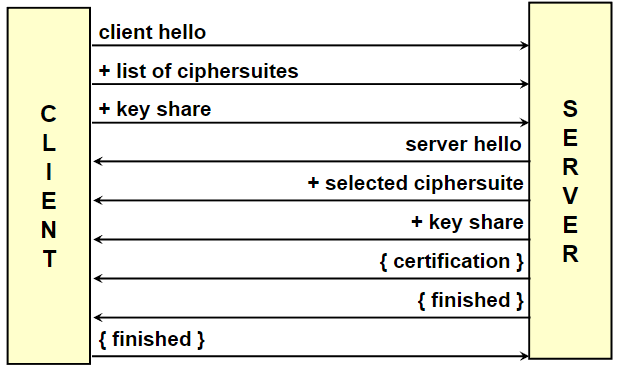
\includegraphics[width=0.8\textwidth]{img/handshakeTLS13.png}
    \caption{TLS 1.3 Handshake}
    \label{fig:tls_handshake}
\end{figure}

\subsection{Notes}
For backward compatibility, TLS-1.2 messages are also sent, and most TLS-1.3 features are in message extensions.
Basically, it's a 1-RTT handshake, that can be reduced to 0-RTT upon resumption of a previous session (or by using true PSK, which is rare)
\\
notation:
\begin{itemize}

    \item\{ data \} = protected by keys derived from a \[sender\]\_handshake\_traffic\_secret
    \item \[ data \] = protected by keys derived from a \[sender\]\_application\_traffic\_secret\_N
\end{itemize}

\subsection{client request}
\textbf{Client Hello:}
\begin{itemize}
    \item client random
    \item highest supported protocol version (note: TLS-1.2 !)
    \item supported ciphersuites and compression methods
    \item session-ID
\end{itemize}
\textbf{contains extensions for key exchange:}
\begin{itemize}
    \item key\_share = client (EC)DHE share
    \item signature\_algorithms = list of supported algorithms
    \item psk\_key\_exchange\_modes = list of supported modes
    \item pre\_shared\_key = list of PSKs offered
\end{itemize}

\subsection{Server Response} %% controllare da slide 

The server response during the TLS-1.3 handshake includes several critical components that facilitate secure communication. 

\begin{itemize}
    \item \textbf{ServerHello}: This message contains:
    \begin{itemize}
        \item \texttt{server random} - a random value generated by the server.
        \item \texttt{selected version} - the TLS version chosen for the session.
        \item \texttt{ciphersuite} - the cipher suite selected for encryption and authentication.
    \end{itemize}

    \item \textbf{Key Exchange}:
    \begin{itemize}
        \item \texttt{key\_share} - the server's (EC)DHE share, which is used for key exchange.
        \item \texttt{pre\_shared\_key} - the selected PSK (Pre-Shared Key).
    \end{itemize}

    \item \textbf{Server Parameters}:
    \begin{itemize}
        \item \{ \textbf{EncryptedExtensions} \} - responses to non-crypto client extensions.
        \item \{ \textbf{CertificateRequest} \} - a request for the client's certificate.
    \end{itemize}

    \item \textbf{Server Authentication}:
    \begin{itemize}
        \item \{ \textbf{Certificate} \} - the server's X.509 certificate (or raw key, RFC-7250).
        \item \{ \textbf{CertificateVerify} \} - a signature covering the entire handshake to validate the server's identity.
        \item \{ \textbf{Finished} \} - a message that contains a MAC (Message Authentication Code) over the entire handshake to ensure integrity.
    \end{itemize}
    
    \item \textbf{Application Data}:
\end{itemize}

\subsection{client finish}

\subsection{Pre Shared Key}
\textbf{PSK} replaces session-ID and session ticket (one or more PSKs agreed in a full handshake and re-used for 
other connections). \\
\textbf{With ECDHE} can be used for forward secrecy. \\
It's also used for OOB, but this is risky (and discouraged) if have insufficient randomness (possible brute force attack). \\

\subsection{0-RTT connection}
\section*{TLS 1.3 - 0-RTT Connections}

In TLS 1.3, when using a Pre-Shared Key (PSK), the client can send \textbf{early data} along with its first message (client request). This early data is protected using a specific key called the \texttt{client\_early\_traffic\_secret}. 

However, 0-RTT does not provide \textbf{forward secrecy}, as the security depends solely on the PSK. This also opens up the possibility of \textbf{replay attacks}. While partial mitigations are feasible, they are complex, especially in the case of multi-instance servers.

\subsection{Incorrect Share}

In TLS 1.3, the client can send a list of (EC)DHE groups that are not supported by the server. In this case, the server will respond with a \textbf{HelloRetryRequest}, and the client must restart the handshake with a different group.
If the newly proposed groups are also unacceptable to the server, the handshake will be aborted, and the server will send an appropriate alert.

\section{TLS and PKI}

PKI needed for server (and optionally) client authentication, unless PSK authentication is adopted. \\
When a peer sends its certificare:
\begin{itemize}
    \item The whole chain is needed (but the root CA - beware!)
    \item Validate the whole chain (not just the EE certificate)
    \item Revocation status needed at each step of the chain
\end{itemize}

To check the revocation staus:
\begin{itemize}
    \item CRL can be used but big size and lengthy look-up
    \item OCSP (faster) can be used but generates privacy problems (leaks client navigation history)
    \item both require one additional network connection and add delay (e.g. for OCSP +300ms median, +1s average)
\end{itemize}

\subsection{TLS and certificate status}

When dealing with TLS and certificate validation, a critical concern arises when the URLs for the Certificate Revocation List (CRL) or the Online Certificate Status Protocol (OCSP) are unreachable. This situation can occur due to \textbf{various reasons}, including:
\begin{itemize}
    \item \textbf{Server Error}: The server hosting the CRL or OCSP service is experiencing issues.
    \item \textbf{Network Error}: Connectivity problems preventing access to the revocation service.
    \item \textbf{Access Blocked by Firewall}: Security policies or insecure channels (common with OCSP) may block access.
\end{itemize}

\textbf{Possible Approaches} to handle these situations:

\begin{itemize}
    \item \textbf{Hard Fail}: The page is not displayed, and a security warning is issued to the user.
    \item \textbf{Soft Fail}: The page is displayed under the assumption that the certificate is valid.
\end{itemize}

Both approaches typically require additional load time while waiting for the connection to timeout, which can affect user experience. Therefore, selecting the appropriate method for certificate status handling is essential for maintaining both security and usability in TLS connections.


\subsubsection{Pushed CRL}
Revoked certificates are often generated by compromised intermediate CA. \\
Browser vendors thus decided to push (some) revoked certificates:
\begin{itemize}
    \item Internet Explorer (with browser update – bad, can be blocked)
    \item Firefox - oneCRL (part of the blocklisting process)
    \item Chrome (also Edge, Opera) - CRLsets
\end{itemize}

%% bash commands
\begin{verbatim}
    $ curl https://firefox.settings.services.mozilla.com/v1/buckets/security-state/collections/onecrl/records > crl.json
    $ jq '[.data[] | {enabled,issuerName,serialNumber} | select(.enabled) | del(.enabled)]' crl.json > crl_short.json
\end{verbatim}

Some articles about the Microsoft certificate problems with Windows XP / Internet Explorer 6:
\begin{itemize}
    \item \href{https://us-cert.cisa.gov/ncas/current-activity/2012/06/04/Unauthorized-Microsoft-Digital-Certificates}{Unauthorized Microsoft Digital Certificates}
    \item \href{https://docs.microsoft.com/en-us/security-updates/SecurityAdvisories/2012/2718704?redirectedfrom=MSDN}{Microsoft Security Advisory 2718704}
\end{itemize}

\section{OCSP stapling}

\subsection{Concept}

Certificate Revocation Lists (CRL) and Online Certificate Status Protocol (OCSP) automatic downloads are often disabled. When a client sends an OCSP request, it creates a \textbf{privacy issue}. Furthermore, pushed CRLs contain only a subset of revoked certificates, and browser behavior in handling these is highly variable.

The solution is \textbf{OCSP stapling}, where the server autonomously obtains the OCSP response and sends it along with its certificate to the client.

\subsection{Implementation}

\textbf{OCSP Stapling} is a TLS extension, and it must be specified in the TLS handshake. The first version is defined in \textbf{RFC 6066} with the extension \texttt{status\_request}, and version 2 is defined in \textbf{RFC 6961} as \texttt{status\_request\_v2}, with the value \texttt{CertificateStatusRequest}.

\subsubsection{How it Works}
The TLS server pre-fetches OCSP responses and provides them to the client during the handshake, as part of the server's certificate message. These OCSP responses are "stapled" to the certificates.

\textbf{Benefit:} This eliminates the client's privacy concern and removes the need for the client to connect to an OCSP responder.

\textbf{Downside:} The freshness of the OCSP responses is a potential issue.

\subsubsection{Client Request for OCSP Stapling}
The TLS client \textbf{MAY} send a \textbf{Certificate Status Request (CSR)} to the server as part of the \texttt{ClientHello} message to request the transfer of OCSP responses in the TLS handshake. If the server receives a \texttt{status\_request\_v2} in the \texttt{ClientHello}, it \textbf{MAY} return OCSP responses for its certificate chain, which are sent in a new message called \texttt{CertificateStatus}.

\subsubsection{Problems and Solutions}
\begin{itemize}
    \item Servers \textbf{MAY} ignore the status request.
    \item Clients \textbf{MAY} decide to continue the handshake even if OCSP responses are not provided.
\end{itemize}

The solution to these problems is the use of \textbf{OCSP Must Staple}, where the server is required to provide OCSP responses with the certificates.

\section{OCSP Must Staple}

In \textbf{OCSP Must Staple}, X.509 certificates for servers \textbf{MAY} include a certificate extension called \texttt{TLSFeatures}, which is identified by the OID \texttt{1.3.6.1.5.5.7.1.24} and defined in \textbf{RFC 7633}. 

This extension informs the client that it \textbf{MUST} receive a valid OCSP response as part of the TLS handshake. If the client does not receive a valid OCSP response, it \textbf{SHOULD} reject the server's certificate. \\

\textbf{Benefits:}
\begin{itemize}
    \item \textbf{Efficiency:} The client does not need to query the OCSP responder directly.
    \item \textbf{Attack Resistance:} It prevents attackers from blocking OCSP responses for a specific client or launching a denial-of-service (DoS) attack against the OCSP responder.
\end{itemize}

\subsection{actors and duties}

The \textbf{CA} must include the \texttt{TLSFeatures} extension into the server's certificates, if requested by the server's owner. \\

The \textbf{OCSP Responder} must:
\begin{itemize}
    \item Be available 24/7 (365x24).
    \item Return valid OCSP responses promptly.
\end{itemize}

The \textbf{TLS client} must:
\begin{itemize}
    \item Send the \texttt{Certificate Status Request (CSR)} extension in the \texttt{ClientHello} message.
    \item Understand the OCSP Must Staple extension if it is present in the server's certificate.
    \item Reject the server's certificate if it does not receive an OCSP stapled response.
\end{itemize}


The \textbf{TLS server} must:
\begin{itemize}
    \item Support OCSP Stapling by prefetching and caching OCSP responses.
    \item Provide an OCSP response during the TLS handshake.
    \item Handle errors in communication with the OCSP responders.
\end{itemize}


The \textbf{TLS server administrators} should:
\begin{itemize}
    \item Configure their servers to use OCSP Stapling.
    \item Request a server certificate with the OCSP Must Staple extension.
\end{itemize}

\textbf{Open Issue:} Duration of OCSP Responses. One potential pitfall is the duration of the OCSP stapled response. For example, Cloudflare OCSP responses last for 7 days.

\section{TLS status}
\begin{itemize}[itemsep=0pt]
    \item F5 telemetry report (October 2021) for the top 1M servers:
    \item 63\% have TLS-1.3 (from 80\% USA to 15\% China and Israel)
    \item 25\% certs use ECDSA and 99\% choose non-RSA handshake
    \item 52\% permit RSA, 2.5\% expired certs, 2\% permit SSL-3
    \item Encryption is abused: 83\% of phishing sites use valid TLS and 80\% of sites are hosted by 3.8\% hosting providers
    \item SSLstrip attacks still successful, so urgent need for HSTS or to completely disable plain HTTP
    \item Cert revocation checking mostly broken, which pushes for very short-lived certs
    \item By TLS fingerprinting, 531 servers potentially match the identity of Trickbot malware servers, and 1,164 match Dridex servers
\end{itemize}

\end{document}